\chapter{Geslachtelijke voortplanting van bloemplanten}\label{ch:b2:angiosperm-reproduction}

Een appelboomgaard is in mei wit van de bloesem en luid van de bijen; in
oktober hangen dezelfde bomen zwaar van de \omterm{def:b2:angiosperm-reproduction:seed}{vruchten}, elke appel met tien
zaden, elk \omterm{def:b2:angiosperm-reproduction:seed}{zaad} een embryonaal boompje gewikkeld in een voedselvoorraad.
Die hele omvorming --- de \omterm{def:b2:angiosperm-reproduction:flower}{bloem}, het \omterm{def:b2:plant-life-cycles:heterospory}{stuifmeel} dat door een insect wordt
gedragen, de buis die door de stijl groeit, de \omterm{prop:b2:angiosperm-reproduction:double}{dubbele bevruchting} die
tegelijk een embryo en zijn voedselvoorraad maakt, het \omterm{def:b2:angiosperm-reproduction:flower}{vruchtbeginsel} dat
opzwelt tot een \omterm{def:b2:angiosperm-reproduction:seed}{vrucht} die gemaakt is om te worden opgegeten --- is de
uitvinding die de bloemplanten in honderd miljoen jaar tot de dominante
planten van het land maakte. Dit hoofdstuk volgt haar van de \omterm{def:b2:angiosperm-reproduction:flower}{bloem} tot het
verspreide \omterm{def:b2:angiosperm-reproduction:seed}{zaad}.

\section{De bloem}

\begin{definition}[De delen van een bloem]\label{def:b2:angiosperm-reproduction:flower}
\index{bloem}\index{meeldraad}\index{vruchtblad}\index{vruchtbeginsel}\index{stempel}
Een \emph{bloem} is een korte scheut waarvan de bladeren zijn omgevormd
tot vier kransen. Buitenaan beschermen de \emph{kelkbladen} (samen de
kelk) de knop; dan volgen de \emph{kroonbladen} (de kroon), die reclame
maken; dan de \emph{meeldraden}, elk een helmdraad met een \emph{helmknop}
met vier stuifmeelzakjes; en in het midden een of meer
\emph{vruchtbladen}, elk dichtgevouwen en vergroeid tot een
\emph{stamper} met een ontvankelijke \emph{stempel}, een \emph{stijl} en
een \emph{vruchtbeginsel} dat de \emph{\omterm{def:b2:plant-life-cycles:heterospory}{zaadbeginsels}} omsluit. Een bloem
met zowel meeldraden als vruchtbladen is \emph{tweeslachtig} (de meeste
soorten); \emph{eenhuizige} planten dragen afzonderlijke mannelijke en
vrouwelijke bloemen op één individu (maïs, eik, hazelaar),
\emph{tweehuizige} soorten op afzonderlijke individuen (hulst, wilg,
dadelpalm). De hele zin van het gesloten vruchtblad --- het kenmerk dat
de bedektzadigen hun naam geeft --- is dat de \omterm{def:b2:plant-life-cycles:heterospory}{zaadbeginsels} ingesloten
zijn: \omterm{def:b2:plant-life-cycles:heterospory}{stuifmeel} bereikt ze nooit rechtstreeks, maar moet er door het
weefsel van de plant naartoe groeien, wat de plant laat kiezen.
\end{definition}

\begin{omfigure}
\begin{tikzpicture}[every node/.style={font=\scriptsize}]
  % receptacle and pedicel
  \draw[thick] (0,-2.6) -- (0,-1.6);
  \draw[thick, fill=omExo!20] (-0.9,-1.6) .. controls (-1.0,-1.0) and (1.0,-1.0) .. (0.9,-1.6) -- cycle;
  % sepals
  \foreach \s in {-1,1} \draw[thick, fill=omExo!45] (0.6*\s,-1.4) .. controls (2.0*\s,-1.2) and (2.6*\s,-0.2) .. (2.8*\s,0.6) .. controls (2.0*\s,0.2) and (1.2*\s,-0.6) .. (0.6*\s,-1.4);
  % petals
  \foreach \s in {-1,1} \draw[thick, fill=omThm!15] (0.5*\s,-1.2) .. controls (1.6*\s,0.4) and (2.2*\s,1.8) .. (1.6*\s,3.0) .. controls (1.0*\s,2.0) and (0.5*\s,0.8) .. (0.5*\s,-1.2);
  % ovary with ovules
  \draw[thick, fill=omDef!12] (0,-0.7) ellipse (0.55 and 0.75);
  \foreach \p in {(-0.22,-0.5),(-0.22,-0.9),(0.22,-0.5),(0.22,-0.9)} \draw[thick, omDef, fill=omDef!40] \p circle (0.11);
  % style and stigma
  \draw[thick, fill=omDef!12] (-0.1,0.05) rectangle (0.1,1.9);
  \draw[thick, fill=omDef!40] (0,2.0) ellipse (0.28 and 0.14);
  % stamens
  \foreach \s in {-1,1} { \draw[thick] (0.35*\s,-1.0) .. controls (0.6*\s,0.2) .. (0.9*\s,1.5); \draw[thick, fill=omProp!60] (0.9*\s,1.6) ellipse (0.14 and 0.32); }
  % labels: right side
  \draw (0.28,2.0) -- (3.2,2.6) node[right] {stempel};
  \draw (0.1,1.2) -- (3.2,1.9) node[right] {stijl};
  \draw (0.55,-0.6) -- (3.2,1.2) node[right] {vruchtbeginsel};
  \draw (0.22,-0.9) -- (3.2,0.5) node[right] {zaadbeginsel};
  \draw (2.6,0.35) -- (3.2,-0.4) node[right] {kelkblad};
  % labels: left side
  \draw (-1.5,2.4) -- (-2.6,2.8) node[left] {kroonblad};
  \draw (-0.95,1.9) -- (-2.6,1.9) node[left] {helmknop};
  \draw (-0.65,0.6) -- (-2.6,0.9) node[left] {helmdraad};
  \draw (0,-2.2) -- (-2.6,-2.2) node[left] {bloembodem en steel};
  \node[anchor=west, align=left] at (5.4,0.5) {stempel + stijl + vruchtbeginsel\\$=$ het vruchtblad (stamper)};
  \node[anchor=west, align=left] at (5.4,-0.8) {helmknop + helmdraad\\$=$ de meeldraad};
\end{tikzpicture}

{\small Een \omterm{def:b2:angiosperm-reproduction:flower}{bloem} in lengtedoorsnede: kelkbladen, kroonbladen, meeldraden
(helmdraad en helmknop) en, in het midden, het \omterm{def:b2:angiosperm-reproduction:flower}{vruchtblad} --- \omterm{def:b2:angiosperm-reproduction:flower}{stempel},
stijl en \omterm{def:b2:angiosperm-reproduction:flower}{vruchtbeginsel} --- dat de \omterm{def:b2:plant-life-cycles:heterospory}{zaadbeginsels} omsluit.}
\end{omfigure}

\begin{omfigure}
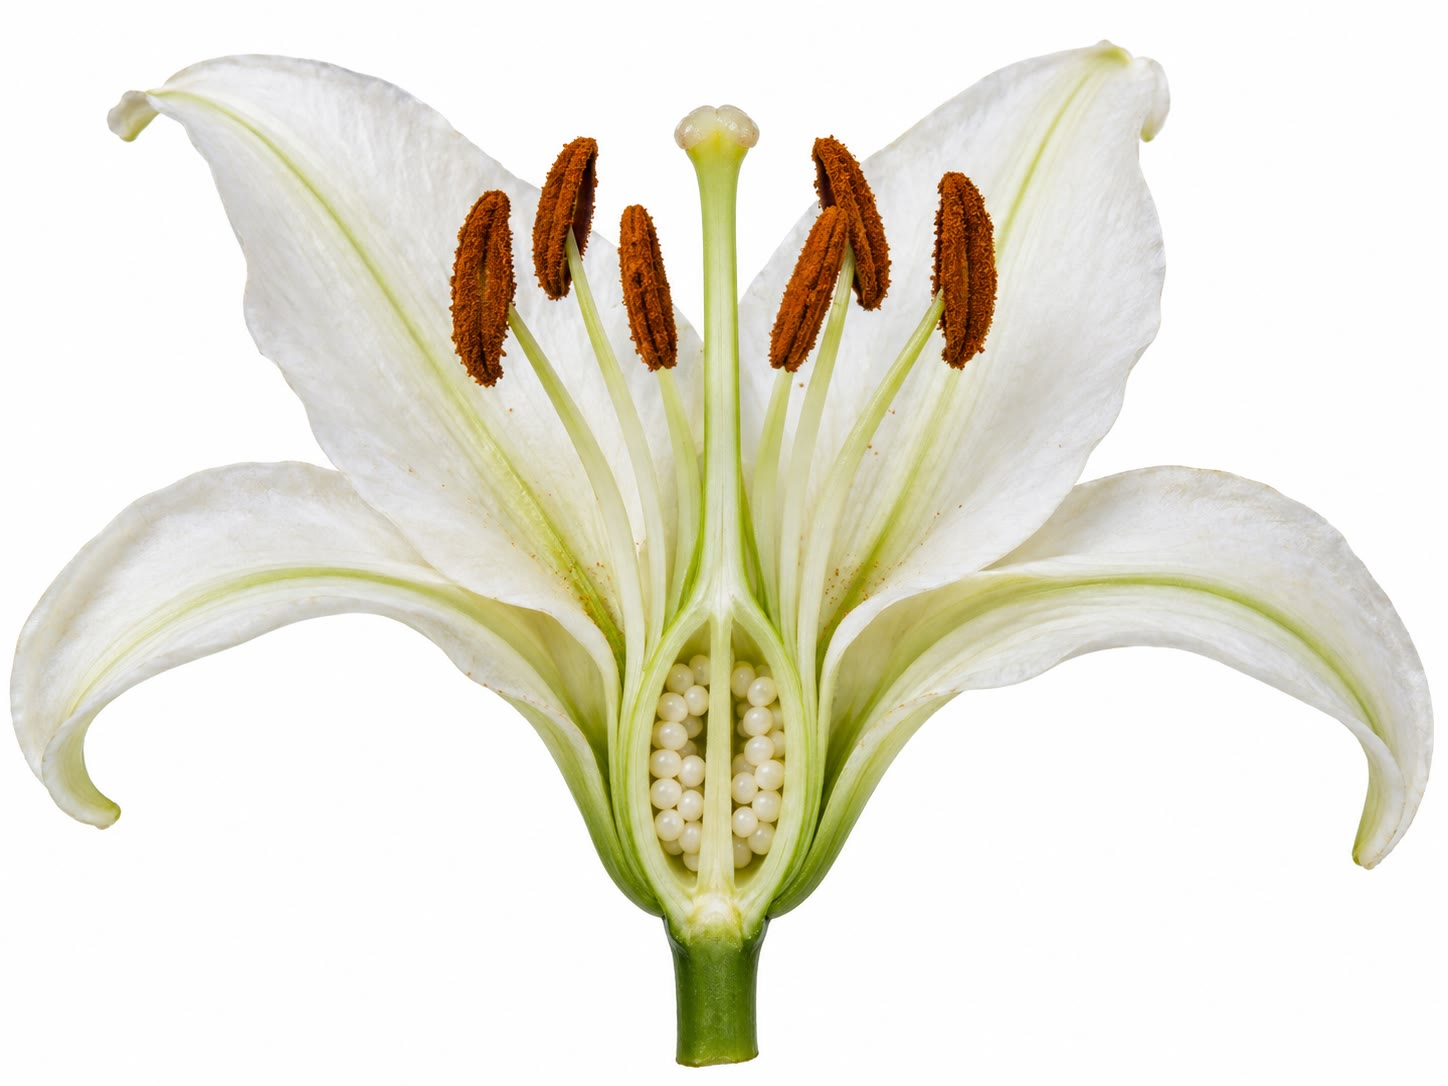
\includegraphics[width=0.55\linewidth]{images/book4/ai/b4-06-lily-dissected.jpg}

{\small Een lelie in de lengte doorgesneden: zes meeldraden met helmknoppen
vol \omterm{def:b2:plant-life-cycles:heterospory}{stuifmeel}, de lange stijl met zijn kleverige \omterm{def:b2:angiosperm-reproduction:flower}{stempel}, en het geopende
\omterm{def:b2:angiosperm-reproduction:flower}{vruchtbeginsel} met de rijen \omterm{def:b2:plant-life-cycles:heterospory}{zaadbeginsels}.}
\end{omfigure}

\section{De twee gametofyten}

\begin{proposition}[Stuifmeel: de mannelijke gametofyt]\label{prop:b2:angiosperm-reproduction:pollen}
\index{stuifmeelkorrel}\index{microsporogenese}\index{sporopollenine}
In elk stuifmeelzakje ondergaan diploïde moedercellen \omterm{def:b2:meiosis-heredity:meiosis}{meiose} tot
tetraden van \emph{\omterm{def:b2:plant-life-cycles:heterospory}{microsporen}}. Elke \omterm{def:b2:plant-life-cycles:heterospory}{microspore} deelt zich één keer,
ongelijk, in een grote \emph{vegetatieve cel} en een kleine
\emph{generatieve cel} die daarin besloten ligt; de generatieve cel deelt
zich, vóór of na de \omterm{def:b2:angiosperm-reproduction:pollination}{bestuiving}, nog één keer in twee
\emph{spermacellen}. De rijpe \emph{\omterm{prop:b2:angiosperm-reproduction:pollen}{stuifmeelkorrel}} is dus een
driecellig \omterm{def:b2:meiosis-heredity:meiosis}{haploïd} organisme --- de hele mannelijke \omterm{def:b2:plant-life-cycles:cycles}{gametofyt} --- van
\qtyrange{10}{100}{\micro m}, afgesloten door een wand waarvan de
buitenste laag van \emph{sporopollenine}, het meest resistente
biologische polymeer dat men kent, gebeeldhouwd is met stekels, poriën
en groeven die kenmerkend zijn voor de soort, en daarom identificeert
\omterm{def:b2:plant-life-cycles:heterospory}{stuifmeel} planten in sedimenten van tientallen miljoenen jaren oud. De
korrel wordt uitgedroogd losgelaten en overleeft uren (grassen) tot weken
(sommige bomen) tot hij een \omterm{def:b2:angiosperm-reproduction:flower}{stempel} bereikt.
\end{proposition}

\begin{omfigure}
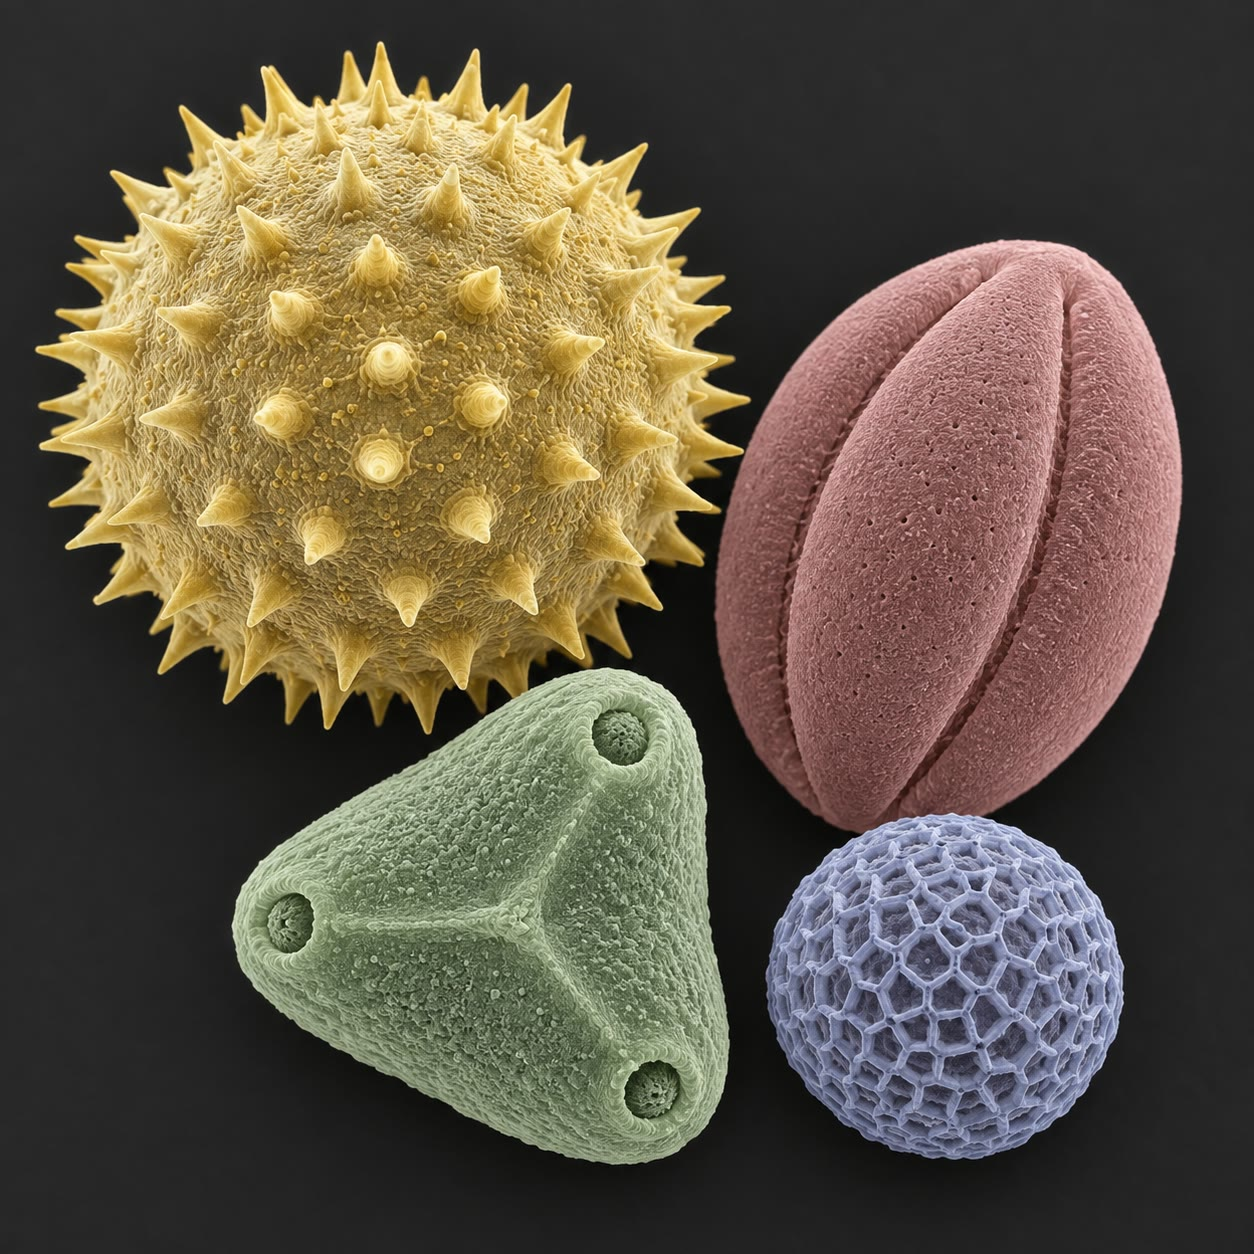
\includegraphics[width=0.45\linewidth]{images/book4/ai/b4-06-pollen-sem.jpg}

{\small \omterm{prop:b2:angiosperm-reproduction:pollen}{Stuifmeelkorrels} onder de rasterelektronenmicroscoop: de wand van
sporopollenine van elke soort heeft een eigen reliëf --- stekels, groeven,
poriën, een netwerk --- waaraan hij te herkennen is.}
\end{omfigure}

\begin{proposition}[De embryozak: de vrouwelijke gametofyt]\label{prop:b2:angiosperm-reproduction:embryosac}
\index{embryozak}\index{megasporogenese}\index{poolkernen}
In elk \omterm{def:b2:plant-life-cycles:heterospory}{zaadbeginsel} ondergaat één diploïde cel van de nucellus \omterm{def:b2:meiosis-heredity:meiosis}{meiose};
drie van de vier \omterm{def:b2:plant-life-cycles:heterospory}{megasporen} degenereren en de vierde groeit door drie
mitosen zonder celdeling uit tot een achtkernige, zevencellige
\emph{\omterm{prop:b2:angiosperm-reproduction:embryosac}{embryozak}}: aan de kant van de micropyle de \emph{eicel},
geflankeerd door twee \emph{synergiden}; aan het andere uiteinde drie
\emph{antipoden}; in het midden een grote \emph{centrale cel} met twee
\emph{\omterm{prop:b2:angiosperm-reproduction:embryosac}{poolkernen}}. Deze zak, omhuld door de nucellus en twee integumenten
met een micropyle, is de hele vrouwelijke \omterm{def:b2:plant-life-cycles:cycles}{gametofyt} --- zeven cellen waar
een \omterm{def:b2:plant-life-cycles:moss}{mos} een plant had. De twee \omterm{prop:b2:angiosperm-reproduction:embryosac}{poolkernen} zijn genetisch identiek aan de
eicel, een feit dat van belang is voor het endosperm.
\end{proposition}

\begin{omfigure}
\begin{tikzpicture}[every node/.style={font=\scriptsize}]
  % pollen grain
  \begin{scope}
    \draw[very thick, omProp!80!black, fill=omProp!15] (0,0) circle (1.1);
    \draw[thick, omProp!80!black] (0,0) circle (0.95);
    \foreach \a in {0,30,...,330} \draw[omProp!80!black, thick] (\a:1.1) -- (\a:1.25);
    \draw[thick, fill=omDef!25] (0.15,-0.2) ellipse (0.55 and 0.4); \node[font=\tiny] at (0.15,-0.2) {vegetatief};
    \draw[thick, fill=omThm!30] (-0.3,0.45) ellipse (0.22 and 0.14); \draw[thick, fill=omThm!30] (0.2,0.5) ellipse (0.22 and 0.14);
    \draw[omThm] (0.0,0.62) -- (0.0,1.5); \node[omThm, anchor=south] at (0.0,1.5) {twee spermacellen};
    \node[below, align=center] at (0,-1.4) {stuifmeelkorrel ($n$)\\3 cellen, wand van sporopollenine};
  \end{scope}
  % ovule with embryo sac
  \begin{scope}[xshift=5.5cm]
    \draw[thick, fill=omExo!25] (0,0) ellipse (1.5 and 2.1);
    \draw[thick, fill=omExo!10] (0,0) ellipse (1.15 and 1.75);
    \fill[white] (-0.3,1.7) rectangle (0.3,2.2); \draw[thick] (-0.3,1.7) -- (-0.3,2.15); \draw[thick] (0.3,1.7) -- (0.3,2.15);
    \draw[thick, fill=white] (0,0) ellipse (0.7 and 1.35);
    % cells: egg + synergids top, central, antipodals bottom
    \draw[thick, fill=omThm!30] (0,0.95) circle (0.17); \node[omThm, anchor=west] at (1.6,1.2) {eicel};
    \draw[thick, fill=omDef!25] (-0.35,1.0) circle (0.14); \draw[thick, fill=omDef!25] (0.35,1.0) circle (0.14); \node[anchor=west] at (1.6,0.75) {twee synergiden};
    \draw[thick, fill=omDef!10] (0,0) ellipse (0.55 and 0.6); \fill[omDef!80!black] (-0.15,0.05) circle (0.09); \fill[omDef!80!black] (0.15,0.05) circle (0.09);
    \node[anchor=west, align=left] at (1.6,0.1) {centrale cel met\\twee poolkernen};
    \foreach \x in {-0.3,0,0.3} \draw[thick, fill=omDef!25] (\x,-1.0) circle (0.13); \node[anchor=west] at (1.6,-1.0) {drie antipoden};
    \draw (0.35,2.0) -- (1.6,2.0) node[right] {micropyle};
    \draw (1.3,-0.9) -- (1.6,-1.6) node[right] {integumenten};
    \draw (0.9,-1.35) -- (1.6,-2.1) node[right] {nucellus};
    \draw (1.6,1.2) -- (0.17,0.95); \draw (1.6,0.75) -- (0.49,1.0); \draw (1.6,0.1) -- (0.55,0.05); \draw (1.6,-1.0) -- (0.43,-1.0);
    \node[below, align=center] at (0,-2.3) {zaadbeginsel met embryozak ($n$)\\7 cellen, 8 kernen};
  \end{scope}
\end{tikzpicture}

{\small De twee \omterm{def:b2:plant-life-cycles:cycles}{gametofyten} van een bloemplant, beide teruggebracht tot
enkele cellen: de driecellige \omterm{prop:b2:angiosperm-reproduction:pollen}{stuifmeelkorrel}, en de zevencellige
\omterm{prop:b2:angiosperm-reproduction:embryosac}{embryozak} in het \omterm{def:b2:plant-life-cycles:heterospory}{zaadbeginsel}.}
\end{omfigure}

\section{Bestuiving}

\begin{definition}[Bestuiving en haar overbrengers]\label{def:b2:angiosperm-reproduction:pollination}
\index{bestuiving}\index{bestuivingssyndroom}\index{nectar}
\emph{Bestuiving} is de overdracht van \omterm{def:b2:plant-life-cycles:heterospory}{stuifmeel} van een helmknop naar een
\omterm{def:b2:angiosperm-reproduction:flower}{stempel}; \emph{zelfbestuiving} binnen één \omterm{def:b2:angiosperm-reproduction:flower}{bloem} of plant,
\emph{kruisbestuiving} tussen planten. \emph{Windbestoven} \omterm{def:b2:angiosperm-reproduction:flower}{bloemen}
(grassen, eiken, berken, weegbree) zijn klein, groen en geurloos, met
grote veervormige \omterm{def:b2:angiosperm-reproduction:flower}{stempels} en enorme hoeveelheden glad, droog \omterm{def:b2:plant-life-cycles:heterospory}{stuifmeel};
hun verhouding van \omterm{def:b2:plant-life-cycles:heterospory}{stuifmeel} tot \omterm{def:b2:plant-life-cycles:heterospory}{zaadbeginsels} loopt op tot een miljoen.
\emph{Door dieren bestoven} \omterm{def:b2:angiosperm-reproduction:flower}{bloemen} betalen hun drager: \emph{nectar}
(suikeroplossing uit nectariën), het \omterm{def:b2:plant-life-cycles:heterospory}{stuifmeel} zelf, oliën, geur; en ze
maken reclame met kleur, vorm en geur die zijn afgestemd op de zintuigen
van de drager --- ultraviolette nectarwijzers voor bijen, die ultraviolet
zien en geen rood; rode buisvormige \omterm{def:b2:angiosperm-reproduction:flower}{bloemen} zonder geur voor kolibries;
witte, sterk geurende, 's nachts opengaande \omterm{def:b2:angiosperm-reproduction:flower}{bloemen} met diepe buizen voor
nachtvlinders; bruine, stinkende \omterm{def:b2:angiosperm-reproduction:flower}{bloemen} voor aasvliegen; stevige, bleke
nachtbloemen voor vleermuizen. Elk zo'n geheel van kenmerken is een
\emph{bestuivingssyndroom}, en de pasvorm tussen \omterm{def:b2:angiosperm-reproduction:flower}{bloem} en bestuiver is het
schoolvoorbeeld van \emph{co-evolutie}: Darwin voorspelde uit de nectarspoor
van \qty{30}{cm} van een orchidee uit Madagaskar een nachtvlinder met een
tong van \qty{30}{cm}, die veertig jaar later werd gevonden.
\end{definition}

\begin{omfigure}
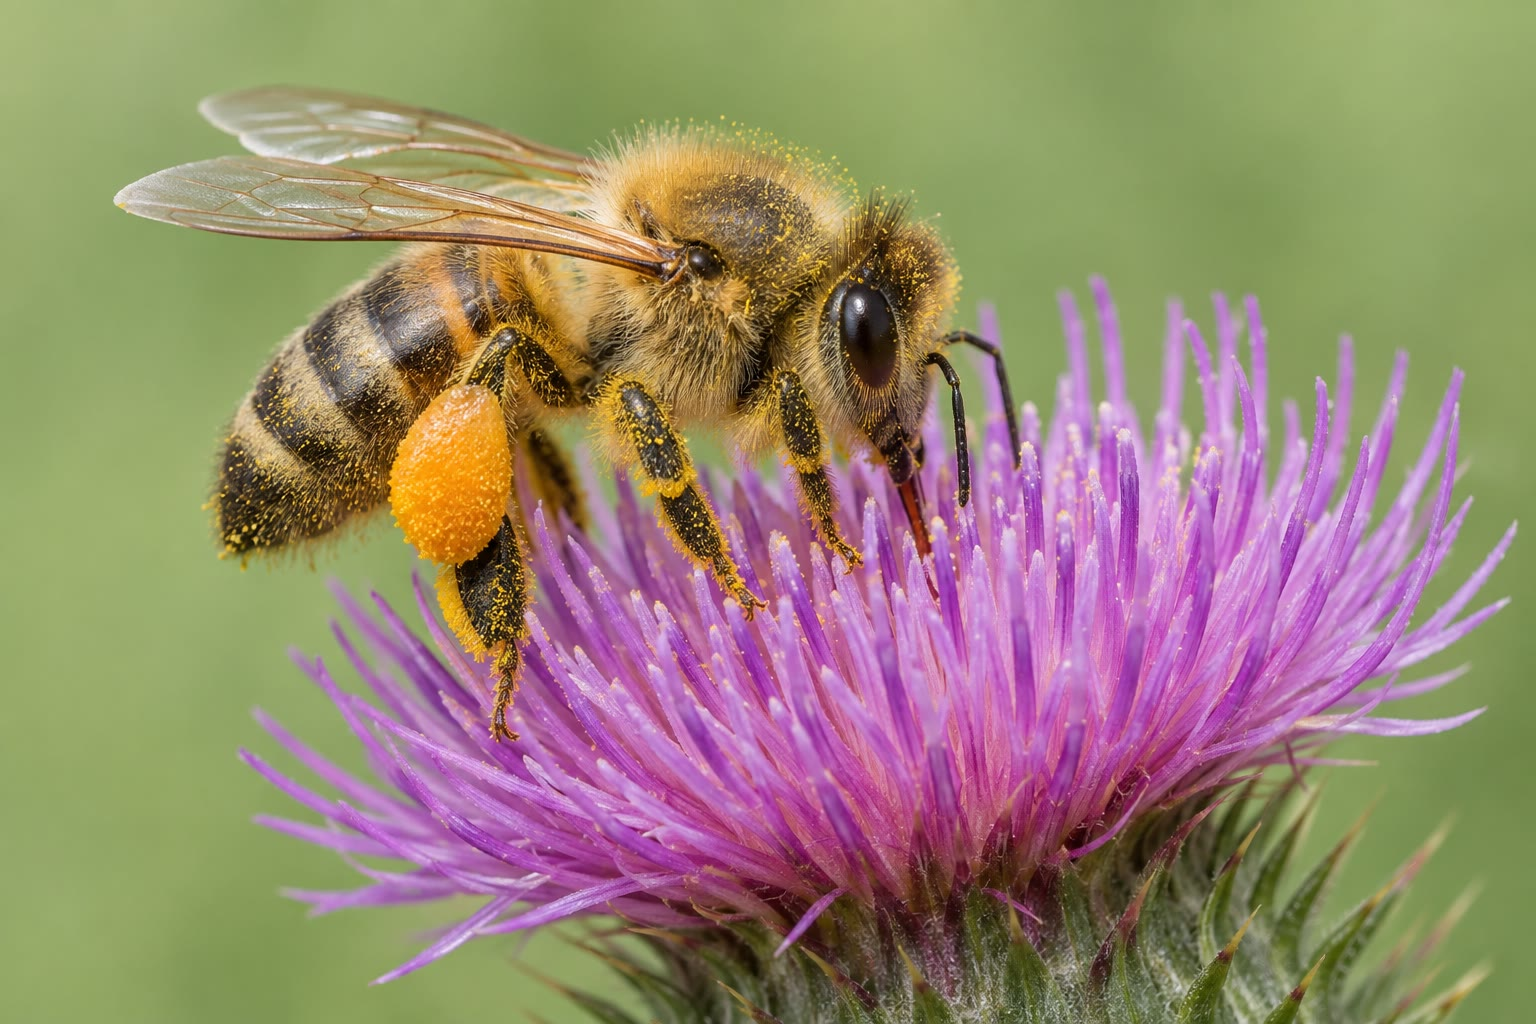
\includegraphics[width=0.58\linewidth]{images/book4/ai/b4-06-bee-on-flower.jpg}

{\small Een honingbij op een distel: \omterm{def:b2:plant-life-cycles:heterospory}{stuifmeel} bestuift haar lichaam en
vult de korfjes aan haar achterpoten; een deel ervan zal de \omterm{def:b2:angiosperm-reproduction:flower}{stempel}
bereiken van de volgende distel die ze bezoekt. Paars, een landingsplatform
en overvloedige \omterm{def:b2:angiosperm-reproduction:pollination}{nectar} vormen het syndroom van de bij.}
\end{omfigure}

\begin{proposition}[Zelfbevruchting vermijden]\label{prop:b2:angiosperm-reproduction:selfing}
\index{zelfincompatibiliteit}\index{heterostylie}\index{dichogamie}
Een tweeslachtige \omterm{def:b2:angiosperm-reproduction:flower}{bloem} zou zichzelf kunnen bevruchten, en veel \omterm{def:b2:angiosperm-reproduction:flower}{bloemen}
doen dat ook (erwten, tarwe, tomaten); maar zelfbevruchting stelt
recessieve schadelijke \omterm{def:b2:meiosis-heredity:vocabulary}{allelen} bloot (\emph{inteeltdepressie}), en de
meeste soorten verhinderen haar. In de tijd: \emph{dichogamie}, waarbij
helmknoppen en \omterm{def:b2:angiosperm-reproduction:flower}{stempel} op verschillende tijdstippen rijp worden
(protandrie bij de meeste schermbloemigen en composieten). In de ruimte:
\emph{herkogamie}, waarbij helmknoppen en \omterm{def:b2:angiosperm-reproduction:flower}{stempel} uit elkaar worden
gehouden, zoals bij de \emph{heterostylie} van sleutelbloemen, waarvan de
langstijlige \omterm{def:b2:angiosperm-reproduction:flower}{bloemen} (lange stijl, lage helmknoppen) en de kortstijlige
\omterm{def:b2:angiosperm-reproduction:flower}{bloemen} (korte stijl, hoge helmknoppen) het \omterm{def:b2:plant-life-cycles:heterospory}{stuifmeel} op verschillende
delen van een insect plaatsen. Biochemisch:
\emph{zelfincompatibiliteit}, een herkenningssysteem waarbij \omterm{def:b2:plant-life-cycles:heterospory}{stuifmeel} dat
een $S$-allel met de stamper deelt, wordt afgewezen. Bij
\emph{gametofytische} incompatibiliteit (appels, kersen, petunia's,
grassen) beslist het eigen haploïde $S$-allel van het \omterm{def:b2:plant-life-cycles:heterospory}{stuifmeel}: een
stamper
$S_1S_2$ houdt buizen $S_1$ en $S_2$ in de stijl tegen, zodat \omterm{def:b2:plant-life-cycles:heterospory}{stuifmeel} van
een plant $S_1S_3$ voor de helft compatibel is en van $S_3S_4$ volledig. Bij
\emph{sporofytische} incompatibiliteit (kolen, zonnebloemen) beslist het
diploïde \omterm{def:b2:meiosis-heredity:vocabulary}{genotype} van de ouder van het \omterm{def:b2:plant-life-cycles:heterospory}{stuifmeel}, op het oppervlak van de
\omterm{def:b2:angiosperm-reproduction:flower}{stempel}. Een zeldzaam $S$-allel is compatibel met bijna elke partner,
zodat selectie tientallen \omterm{def:b2:meiosis-heredity:vocabulary}{allelen} in een populatie in stand houdt.
\end{proposition}
\begin{proof}[Bewijsmateriaal]
Darwin (1862, 1877) kruiste sleutelbloemen met de hand: \omterm{def:b2:plant-life-cycles:heterospory}{stuifmeel} van een
kortstijlige \omterm{def:b2:angiosperm-reproduction:flower}{bloem} op een langstijlige \omterm{def:b2:angiosperm-reproduction:flower}{stempel} (een ``legitieme''
verbinding) gaf volle doosvruchten; langstijlig op langstijlig of
kortstijlig op kortstijlig (``illegitiem'') gaf weinig of geen zaden,
hoewel de planten gezond waren en het \omterm{def:b2:plant-life-cycles:heterospory}{stuifmeel} levend. Hij concludeerde
dat de twee vormen wederzijds op kruising waren aangepast en tegen
zelfbevruchting beschermd, en door in duizenden kruisingen de zaden per
doosvrucht te tellen, mat hij de kosten van zelfbevruchting bij tientallen
soorten: zelfbevruchte nakomelingen waren kleiner, lichter en minder
vruchtbaar, generatie na generatie.
\end{proof}

\begin{omfigure}
\begin{tikzpicture}[every node/.style={font=\scriptsize}]
  % pistil S1S2 with pollen tubes
  \draw[thick, fill=omDef!10] (-0.5,0) rectangle (0.5,3.2);
  \draw[thick, fill=omDef!30] (0,3.3) ellipse (0.7 and 0.2);
  \draw[thick, fill=omDef!12] (0,-0.6) ellipse (0.9 and 0.7);
  \node at (0,-0.6) {vruchtbeginsel};
  \node[anchor=east] at (-1.1,3.3) {stempel van een plant $S_1S_2$};
  % pollen grains
  \draw[thick, fill=omThm!40] (-0.35,3.75) circle (0.13); \node[omThm, left] at (-0.5,3.75) {$S_1$};
  \draw[thick, fill=omThm!40] (0,3.75) circle (0.13); \node[omThm, anchor=south] at (0,3.92) {$S_2$};
  \draw[thick, fill=omExo!70!black] (0.35,3.75) circle (0.13); \node[right] at (0.5,3.75) {$S_3$};
  % tubes: S1 and S2 stop in the style, S3 reaches the ovary
  \draw[thick, omThm] (-0.35,3.3) -- (-0.35,2.3); \node[omThm, left, align=right] at (-0.55,2.3) {buis $S_1$\\tegengehouden};
  \draw[thick, omThm] (0,3.3) -- (0,2.0);
  \draw[thick, omExo!70!black] (0.35,3.3) -- (0.35,-0.2) -- (0.2,-0.5);
  \node[right, align=left] at (0.55,0.9) {buis $S_3$\\bereikt een zaadbeginsel};
  \node[anchor=west, align=left, text width=6cm] at (3.2,3.2) {gametofytische zelfincompatibiliteit: een stuifmeelbuis waarvan het eigen $S$-allel overeenkomt met een van beide allelen van de stamper, wordt in de stijl tegengehouden};
  \node[anchor=west, align=left, text width=6cm] at (3.2,1.4) {stuifmeel van een plant $S_1S_2$: 0 compatibel\\van $S_1S_3$: de helft\\van $S_3S_4$: alles};
\end{tikzpicture}

{\small Gametofytische zelfincompatibiliteit. Op een stamper $S_1S_2$
worden buizen met $S_1$ of $S_2$ in de stijl tegengehouden; een buis met
$S_3$ groeit door tot het \omterm{def:b2:angiosperm-reproduction:flower}{vruchtbeginsel}.}
\end{omfigure}

\section{Bevruchting}

\begin{theorem}[De stuifmeelbuis]\label{thm:b2:angiosperm-reproduction:tube}
\index{stuifmeelbuis}
Een \omterm{prop:b2:angiosperm-reproduction:pollen}{stuifmeelkorrel} op een compatibele \omterm{def:b2:angiosperm-reproduction:flower}{stempel} neemt weer water op en
vormt een \emph{\omterm{thm:b2:angiosperm-reproduction:tube}{stuifmeelbuis}}: de vegetatieve cel verlengt zich door
topgroei, waarbij aan de top nieuwe wand wordt afgezet met een snelheid
van \qtyrange{0.1}{1}{cm/h}, en baant zich verterend een weg door het
geleidende weefsel van de stijl, waarvan ze zich voedt. De buis draagt de
twee spermacellen aan haar top; het laatste stuk wordt ze geleid door
peptiden die de synergiden uitscheiden, ze gaat het \omterm{def:b2:plant-life-cycles:heterospory}{zaadbeginsel} binnen
via de micropyle, barst open in een van de synergiden en laat de
spermacellen vrij. Een buis die een stijl met lengte $L$ met snelheid
$v$ doorkruist, doet daar $L/v$ over: enkele uren bij een kers, een volle
dag bij maïs, waarvan de ``zijden draden'' stijlen van \qty{20}{cm} lang
zijn. De levensvatbaarheid van het \omterm{def:b2:plant-life-cycles:heterospory}{stuifmeel} zet een klok in gang:
\omterm{def:b2:plant-life-cycles:heterospory}{stuifmeel} van grassen sterft binnen uren, dus moet een \omterm{def:b2:angiosperm-reproduction:flower}{stempel} snel
worden bereikt.
\end{theorem}
\begin{proof}
De tijd is de lengte gedeeld door de groeisnelheid; voor maïs geeft
\qty{20}{cm} bij \qty{1}{cm/h} \qty{20}{h}. De buis zelf bestaat vrijwel
geheel uit wand en een dun laagje cytoplasma achter de top, zodat de
reserves van de vegetatieve cel, plus wat ze uit de stijl opneemt,
volstaan voor een lengte van duizend keer de diameter van de korrel.
\end{proof}

\begin{proposition}[Dubbele bevruchting]\label{prop:b2:angiosperm-reproduction:double}
\index{dubbele bevruchting}\index{endosperm}
Van de twee spermacellen die de buis aflevert, versmelt de ene met de
eicel tot de diploïde \emph{zygote}, waaruit het embryo groeit; de andere
versmelt met de centrale cel en haar twee \omterm{prop:b2:angiosperm-reproduction:embryosac}{poolkernen} tot een
\emph{triploïde} kern ($3n$: twee maternale genomen, één paternaal),
waaruit het \emph{endosperm} groeit --- een voedingsweefsel dat het \omterm{def:b2:angiosperm-reproduction:seed}{zaad}
vult met zetmeel, olie en eiwit. Beide bevruchtingen vinden binnen enkele
minuten na elkaar plaats; bij de meeste soorten slaagt geen van beide
zonder de andere, zodat een plant alleen de zaden bevoorraadt die een
embryo dragen. Het endosperm is het weefsel dat de mensheid voedt: de
\omterm{def:b2:angiosperm-reproduction:flower}{bloem} van tarwe en rijst, het meel van maïs, het wit van een kokosnoot
zijn triploïd endosperm. Bij naaktzadigen is de voedselvoorraad van het
\omterm{def:b2:angiosperm-reproduction:seed}{zaad} de vrouwelijke \omterm{def:b2:plant-life-cycles:cycles}{gametofyt}, opgebouwd vóór de bevruchting, of er nu een
embryo volgt of niet; het endosperm van de bedektzadige wordt op bestelling
gemaakt.
\end{proposition}
\begin{proof}[Bewijsmateriaal]
Nawaschin (1898), die de \omterm{thm:b2:angiosperm-reproduction:tube}{stuifmeelbuis} van een lelie en een kievitsbloem
onder de microscoop tot in de \omterm{prop:b2:angiosperm-reproduction:embryosac}{embryozak} volgde, zag beide spermakernen de
buis verlaten, de ene de eicel binnengaan en de andere met de \omterm{prop:b2:angiosperm-reproduction:embryosac}{poolkernen}
versmelten; Guignard bevestigde het het jaar erna bij andere soorten. De
triploïdie van het endosperm volgde uit chromosoomtellingen, en de
genetische gevolgen ervan --- een endosperm van een maïskorrel dat de
kenmerken van de stuifmeelouder vertoont (\emph{xenie}), in de verhouding
twee maternale doses op één paternale --- waren veredelaars van maïs al
lang eerder opgevallen.
\end{proof}

\begin{omfigure}
\begin{tikzpicture}[every node/.style={font=\scriptsize}, >=stealth]
  \node[draw, rounded corners, fill=omProp!15, align=center] (sp) at (0,2) {spermacel 1 ($n$)};
  \node[draw, rounded corners, fill=omProp!15, align=center] (sp2) at (0,0) {spermacel 2 ($n$)};
  \node[draw, rounded corners, fill=omThm!15, align=center] (egg) at (4,2) {eicel ($n$)};
  \node[draw, rounded corners, fill=omDef!15, align=center] (cc) at (4,0) {centrale cel\\twee poolkernen ($n + n$)};
  \node[draw, rounded corners, fill=omThm!30, align=center] (zyg) at (8.6,2) {zygote ($2n$)\\$\to$ embryo};
  \node[draw, rounded corners, fill=omDef!30, align=center] (endo) at (8.6,0) {endospermkern ($3n$)\\$\to$ endosperm, de voedselvoorraad};
  \draw[->, thick] (sp) -- (egg); \draw[->, thick] (egg) -- (zyg);
  \draw[->, thick] (sp2) -- (cc); \draw[->, thick] (cc) -- (endo);
  \node[anchor=south] at (2,2.5) {bevruchting 1};
  \node[anchor=south] at (2,0.5) {bevruchting 2};
  \node[anchor=north, align=center] at (4.3,-0.9) {één stuifmeelbuis, twee spermacellen, twee versmeltingen: het embryo en zijn voedselvoorraad worden samen gemaakt};
\end{tikzpicture}

{\small \omterm{prop:b2:angiosperm-reproduction:double}{Dubbele bevruchting}: de ene spermacel maakt de diploïde zygote,
de andere het triploïde endosperm.}
\end{omfigure}

\section{Zaad en vrucht}

\begin{definition}[Van zaadbeginsel tot zaad, van vruchtbeginsel tot vrucht]\label{def:b2:angiosperm-reproduction:seed}
\index{zaad}\index{vrucht}\index{zaadlob}\index{kiemrust}
De zygote deelt zich in een suspensor, die het embryo het endosperm in
duwt, en een eigenlijk embryo dat een bolvormig, hartvormig en
torpedovormig stadium doorloopt terwijl het de wortel- en scheutpool
aanlegt en een of twee \emph{zaadlobben} (kiembladen) --- het onderscheid
tussen eenzaadlobbigen en tweezaadlobbigen. Bij veel tweezaadlobbigen
(bonen, erwten) nemen de groeiende zaadlobben het endosperm op en worden
ze zelf de voedselvoorraad; bij granen en de meeste eenzaadlobbigen blijft
het endosperm bestaan en is de enige zaadlob een zuigorgaan. De
integumenten verharden tot de \emph{zaadhuid}; het zaad droogt uit tot
\qtyrange{5}{15}{\%} water, het metabolisme stopt, en het gaat in
\emph{kiemrust}, die pas eindigt wanneer een signaal --- water, kou,
licht, vuur, de doorgang door een darm --- zegt dat het seizoen gunstig
is. Intussen groeit de wand van het \omterm{def:b2:angiosperm-reproduction:flower}{vruchtbeginsel} uit tot de
\emph{vrucht}, waarvan de vorm een verspreidingsstrategie is: droge
vruchten die openspringen (peulen, doosvruchten) of niet (graankorrels,
noten, gevleugelde nootjes), vlezige vruchten die worden gegeten (bessen,
steenvruchten met een pit, de appel, waarvan het vruchtvlees bloembodem
is); het zaad passeert het dier onbeschadigd, met een opgeruwde zaadhuid,
en wordt met mest kilometers verder afgezet.
\end{definition}
\begin{proof}[Bewijsmateriaal]
De graankorrel laat zien hoe kieming wordt gestuurd. Het embryo scheidt,
wanneer het water opneemt, gibberelline af in het omringende endosperm;
de buitenste laag van het endosperm, de aleuronlaag, reageert door
$\alpha$-amylase te maken en uit te scheiden, dat het zetmeel verteert tot
suikers die het embryo opneemt. Halve korrels zonder embryo maken geen
amylase; voeg er gibberelline aan toe en ze doen het wel (Paleg, Yomo,
1960); het hormoon werkt door het amylasegen aan te schakelen, een van de
eerste gevallen waarin een plantenhormoon tot een gen werd herleid.
Bierbrouwers gebruiken het proces al duizenden jaren: mouten is gerst die
men laat kiemen en daarna droogt.
\end{proof}

\begin{omfigure}
\begin{tikzpicture}[every node/.style={font=\scriptsize}]
  % embryogenesis stages
  \foreach \x/\lab in {0/{zygote}, 1.6/{twee cellen}, 3.4/{bolvormig}, 5.6/{hartvormig}, 8.2/{torpedovormig}} \node[below] at (\x,-1.1) {\lab};
  \draw[thick, fill=omThm!25] (0,-0.2) circle (0.22);
  \draw[thick, fill=omThm!25] (1.6,0.0) circle (0.2); \draw[thick, fill=omDef!15] (1.6,-0.45) circle (0.14);
  \draw[thick, fill=omThm!25] (3.4,0.1) circle (0.45); \foreach \y in {-0.5,-0.75,-1.0} \draw[thick, fill=omDef!15] (3.4,\y) circle (0.1);
  \draw[thick, fill=omThm!25] (5.6,0.0) .. controls (4.9,1.0) and (5.2,-0.6) .. (5.6,-0.6) .. controls (6.0,-0.6) and (6.3,1.0) .. (5.6,0.0);
  \draw[thick, fill=omThm!25] (5.15,0.5) circle (0.32); \draw[thick, fill=omThm!25] (6.05,0.5) circle (0.32);
  \foreach \y in {-0.75,-1.0} \draw[thick, fill=omDef!15] (5.6,\y) circle (0.09);
  \draw[thick, fill=omThm!25] (8.2,-0.2) ellipse (0.3 and 0.75);
  \draw[thick, fill=omThm!25] (7.75,0.9) .. controls (7.4,1.6) and (7.9,1.9) .. (8.05,0.55) -- cycle;
  \draw[thick, fill=omThm!25] (8.65,0.9) .. controls (9.0,1.6) and (8.5,1.9) .. (8.35,0.55) -- cycle;
  \node[omDef!80!black, anchor=west] at (9.3,-0.9) {suspensor (blauw)};
  \node[omThm, anchor=west] at (9.3,0.9) {zaadlobben};
  \node[anchor=west] at (9.3,-0.2) {wortelpool onderaan};
\end{tikzpicture}

{\small Embryogenese bij een tweezaadlobbige: de zygote deelt zich in een
embryo en een suspensor; het bolvormige embryo wordt hartvormig wanneer de
twee zaadlobben verschijnen, en daarna torpedovormig wanneer de
wortel-scheutas zich verlengt.}
\end{omfigure}

\begin{omfigure}
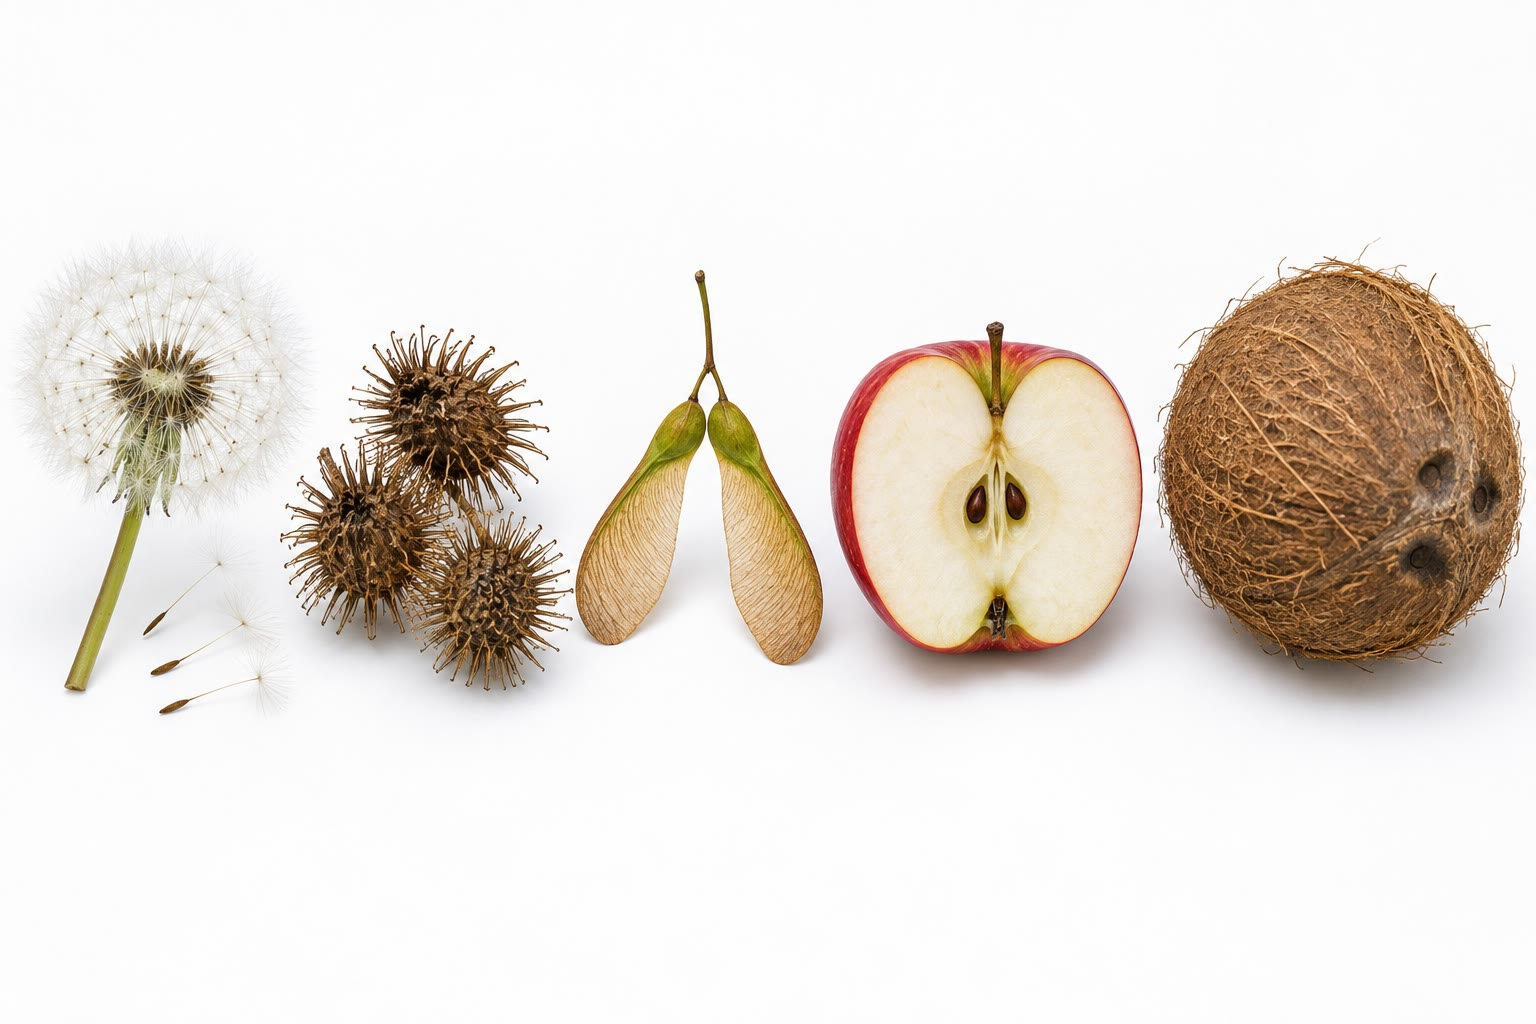
\includegraphics[width=0.62\linewidth]{images/book4/ai/b4-06-fruits-seeds.jpg}

{\small \omterm{def:b2:angiosperm-reproduction:seed}{Vruchten} gebouwd voor verspreiding: parachutes (paardenbloem),
haakjes (klit), vleugels (esdoorn), vruchtvlees voor een dier (appel), en
een drijvende bolster voor de zee (kokosnoot).}
\end{omfigure}

\begin{example}[Verspreidingsafstanden]\label{ex:b2:angiosperm-reproduction:dispersal}
Een nootje van een paardenbloem daalt met zijn parachute met
\qty{0.3}{m/s}; vanaf \qty{0.3}{m} vliegt het in een wind van \qty{3}{m/s}
\qty{3}{m} ver, en in een thermiekbel honderden. Een gevleugeld nootje van
een esdoorn draait als een wentelwiek omlaag met
\qty{1}{m/s} vanaf \qty{15}{m}: \qty{45}{m}. Een kersenpit die een vogel
laat vallen na een vlucht van twintig minuten met \qty{10}{m/s}: tot
\qty{12}{km}. De eikels van een eik vallen aan zijn voet, tenzij een
Vlaamse gaai ze meeneemt, wat hij bij duizenden doet, een kilometer en
verder, en een tiende ervan vergeet: de eiken die na de laatste ijstijd
Europa herkoloniseerden, schoven met honderden meters per jaar naar het
noorden, veel sneller dan een eikel rolt, en het waren de vogels die ze
verplaatsten.
\end{example}

\section{Opgaven}

\begin{exercise}[$\star$]\label{exo:b2:angiosperm-reproduction:1}
Noem de vier kransen van een \omterm{def:b2:angiosperm-reproduction:flower}{bloem} en de delen van een \omterm{def:b2:angiosperm-reproduction:flower}{meeldraad} en van
een \omterm{def:b2:angiosperm-reproduction:flower}{vruchtblad}. Welke delen zijn diploïde \omterm{def:b2:plant-life-cycles:cycles}{sporofyt}, welke haploïde
\omterm{def:b2:plant-life-cycles:cycles}{gametofyt}?
\end{exercise}

\begin{exercise}[$\star$]\label{exo:b2:angiosperm-reproduction:2}
Geef de ploïdie van: een \omterm{def:b2:plant-life-cycles:heterospory}{microspore}, de vegetatieve cel, een spermacel,
de eicel, een poolkern, de zygote, het endosperm, de \omterm{def:b2:angiosperm-reproduction:seed}{zaadhuid}, de
vruchtwand.
\end{exercise}

\begin{exercise}[$\star$]\label{exo:b2:angiosperm-reproduction:3}
Noem vijf kenmerken van een windbestoven \omterm{def:b2:angiosperm-reproduction:flower}{bloem} en vijf van een door bijen
bestoven \omterm{def:b2:angiosperm-reproduction:flower}{bloem}, en geef bij elk een plant.
\end{exercise}

\begin{exercise}[$\star$]\label{exo:b2:angiosperm-reproduction:4}
Wat is \omterm{prop:b2:angiosperm-reproduction:double}{dubbele bevruchting}, en wat maakt elk van de twee versmeltingen?
Waarom kan men het endosperm ``op bestelling gemaakt'' noemen?
\end{exercise}

\begin{exercise}[$\star\star$]\label{exo:b2:angiosperm-reproduction:5}
Een zijden draad van maïs is \qty{25}{cm} lang en een \omterm{thm:b2:angiosperm-reproduction:tube}{stuifmeelbuis} groeit
met \qty{1.2}{cm/h}. Hoelang duurt het van \omterm{def:b2:angiosperm-reproduction:pollination}{bestuiving} tot bevruchting?
Een pluim geeft \omterm{def:b2:plant-life-cycles:heterospory}{stuifmeel} af van dag 0 tot dag 7, en de zijden draden van
de plant verschijnen van dag 5 tot dag 12, elke dag een achtste ervan; een
draad vangt alleen \omterm{def:b2:plant-life-cycles:heterospory}{stuifmeel} zolang er \omterm{def:b2:plant-life-cycles:heterospory}{stuifmeel} wordt afgegeven. Welk
deel van de draden wordt bestoven?
\end{exercise}

\begin{exercise}[$\star\star$]\label{exo:b2:angiosperm-reproduction:6}
Welk deel van het \omterm{def:b2:plant-life-cycles:heterospory}{stuifmeel} is bij gametofytische zelfincompatibiliteit
compatibel in de kruisingen $S_1S_2\times S_1S_2$, $S_1S_2\times
S_1S_3$, $S_1S_2\times S_3S_4$ (stamper eerst vermeld)? Geef de
\omterm{def:b2:meiosis-heredity:vocabulary}{genotypen} van de nakomelingen van de tweede kruising.
\end{exercise}

\begin{exercise}[$\star\star$]\label{exo:b2:angiosperm-reproduction:7}
Welk deel van willekeurig \omterm{def:b2:plant-life-cycles:heterospory}{stuifmeel} is in een populatie met $n$ even
frequente $S$-allelen compatibel met een gegeven plant? Leg uit waarom een
nieuw $S$-allel dat door \omterm{def:b2:genome-diversification:mutation}{mutatie} ontstaat zich verspreidt, en wat dit
voorspelt voor het aantal \omterm{def:b2:meiosis-heredity:vocabulary}{allelen}.
\end{exercise}

\begin{exercise}[$\star\star$]\label{exo:b2:angiosperm-reproduction:8}
Een maïsplant die \omterm{def:b2:meiosis-heredity:vocabulary}{heterozygoot} $Yy$ is (geel endosperm \omterm{def:b2:meiosis-heredity:vocabulary}{dominant}), wordt
zelfbestoven. Geef de endospermgenotypen van haar korrels en hun
verhoudingen, bedenkend dat de twee \omterm{prop:b2:angiosperm-reproduction:embryosac}{poolkernen} identiek zijn.
Welk deel van de korrels is geel? En als de plant wordt bestoven
door een plant $yy$?
\end{exercise}

\begin{exercise}[$\star\star$]\label{exo:b2:angiosperm-reproduction:9}
Beschrijf het aleuronexperiment en leg uit wat het aantoont over
(a) de rol van het embryo, (b) de rol van gibberelline, (c) de
plaats van de amylasesynthese. Waarom is een halve korrel zonder embryo
de essentiële controle?
\end{exercise}

\begin{exercise}[$\star\star\star$]\label{exo:b2:angiosperm-reproduction:10}
Vergelijk de wind- en de dierstrategie in kosten: een windbestoven
plant maakt $10^{6}$ korrels per \omterm{def:b2:plant-life-cycles:heterospory}{zaadbeginsel} van elk \qty{1}{\micro g};
een door dieren bestoven plant maakt $10^{3}$ korrels per \omterm{def:b2:plant-life-cycles:heterospory}{zaadbeginsel} van
elk \qty{1}{\micro g} plus \qty{5}{mg} nectarsuiker per \omterm{def:b2:angiosperm-reproduction:flower}{bloem}
met tien \omterm{def:b2:plant-life-cycles:heterospory}{zaadbeginsels}. Bereken de voortplantingskosten per \omterm{def:b2:plant-life-cycles:heterospory}{zaadbeginsel}
in beide gevallen (neem voor \omterm{def:b2:plant-life-cycles:heterospory}{stuifmeel} en suiker dezelfde energie per
gram), en leg uit waarom windbestuiving toch blijft bestaan.
\end{exercise}

\begin{exercise}[$\star\star\star$]\label{exo:b2:angiosperm-reproduction:11}
Leg met de getallen van \cref{ex:b2:angiosperm-reproduction:dispersal}
uit waarom een vlezige \omterm{def:b2:angiosperm-reproduction:seed}{vrucht} voor een boom de kosten waard is, ook al
verteert het dier het vruchtvlees en laat het de meeste zaden vallen waar
ze niet kunnen groeien.
\end{exercise}

\begin{exercise}[$\star\star\star$]\label{exo:b2:angiosperm-reproduction:12}
``Het gesloten \omterm{def:b2:angiosperm-reproduction:flower}{vruchtblad} is de reden waarom bloemplanten het land
beheersen.'' Bespreek: wat de insluiting van het \omterm{def:b2:plant-life-cycles:heterospory}{zaadbeginsel} mogelijk
maakt (keuze van \omterm{def:b2:plant-life-cycles:heterospory}{stuifmeel}, incompatibiliteit, de \omterm{def:b2:angiosperm-reproduction:seed}{vrucht}) en wat ze kost.
\end{exercise}

\section{Vraagstuk: een boomgaard en een akker}

\begin{problem}[{Weekendvraagstuk --- de bestuiving van een appelboomgaard,
gepland rond zelfincompatibiliteit, en de bevruchting en opbrengst van een
maïsakker, berekend uit het stuifmeel dat hij maakt, met als besluit de
vruchtzetting van de boomgaard en het aantal maïskorrels van de akker}]
\label{pb:b2:angiosperm-reproduction:1}
De appel is gametofytisch zelfincompatibel. Een boomgaard telt drie
rassen: A ($S_1S_2$), B ($S_1S_3$), C ($S_3S_4$). Een \omterm{def:b2:angiosperm-reproduction:flower}{bloem} heeft vijf
\omterm{def:b2:angiosperm-reproduction:flower}{vruchtbladen} met elk twee \omterm{def:b2:plant-life-cycles:heterospory}{zaadbeginsels}, en een \omterm{def:b2:angiosperm-reproduction:seed}{vrucht} die minder dan vijf
zaden zet, wordt door de boom afgestoten. Een bijenbezoek brengt \num{100}
\omterm{prop:b2:angiosperm-reproduction:pollen}{stuifmeelkorrels} op een \omterm{def:b2:angiosperm-reproduction:flower}{stempel}; elke compatibele korrel heeft kans $0.1$
om een nog niet bezet \omterm{def:b2:plant-life-cycles:heterospory}{zaadbeginsel} te bevruchten. Een boom draagt
\num{5000} \omterm{def:b2:angiosperm-reproduction:flower}{bloemen} en heeft \num{250} \omterm{def:b2:angiosperm-reproduction:seed}{vruchten} nodig voor een volle oogst.
Maïs: een pluim geeft over \num{7} dagen
$10^{7}$ korrels af; de akker telt \num{8} planten per
vierkante meter; een plant draagt één kolf met \num{600} zijden draden;
een draad biedt \qty{1e-4}{m^2} aan vallend \omterm{def:b2:plant-life-cycles:heterospory}{stuifmeel}; \omterm{def:b2:plant-life-cycles:heterospory}{stuifmeel} daalt met
\qty{0.25}{m/s}; een maïskorrel bevat \qty{0.3}{g} endosperm.

\medskip
\noindent\textbf{Deel I --- Compatibiliteit.}
\begin{enumerate}
  \item Geef voor \omterm{def:b2:plant-life-cycles:heterospory}{stuifmeel} van elk ras op een stamper van A de
        compatibele fractie $f$.
  \item Idem voor stampers van B en van C.
  \item Een bij die van een boom van B komt, brengt 100 korrels op een
        \omterm{def:b2:angiosperm-reproduction:flower}{stempel} van A: hoeveel zijn er compatibel, en hoeveel \omterm{def:b2:plant-life-cycles:heterospory}{zaadbeginsels}
        worden naar verwachting bevrucht (verwaarloos verzadiging)?
  \item Idem voor een bij van C, en van een andere A.
  \item Welke \omterm{def:b2:angiosperm-reproduction:seed}{vruchten} blijven hangen? Wat is het risico van een boomgaard
        met alleen ras A?
  \item Een blok bomen van A is omringd door bomen van C; de helft van de
        bijenbezoeken aan A komt van C. Als elke \omterm{def:b2:angiosperm-reproduction:flower}{bloem} één bezoek krijgt,
        welk deel van de \omterm{def:b2:angiosperm-reproduction:flower}{bloemen} van A zet dan \omterm{def:b2:angiosperm-reproduction:seed}{vrucht}, en hoeveel \omterm{def:b2:angiosperm-reproduction:seed}{vruchten}
        per boom? Is de oogst vol?
  \item Waarom planten boomgaarden er een sierappel tussen die wekenlang
        bloeit, en waarom moeten zijn $S$-allelen worden gecontroleerd?
\end{enumerate}

\medskip
\noindent\textbf{Deel II --- \omterm{def:b2:plant-life-cycles:heterospory}{Stuifmeel} boven de maïsakker.}
\begin{enumerate}[resume]
  \item Bereken het \omterm{def:b2:plant-life-cycles:heterospory}{stuifmeel} dat per vierkante meter akker per seconde
        vrijkomt, gemiddeld over de zeven dagen.
  \item In de stationaire toestand is de flux van neerdalend \omterm{def:b2:plant-life-cycles:heterospory}{stuifmeel}
        gelijk aan de afgifte. Bereken de stuifmeelconcentratie in de lucht
        (korrels per kubieke meter).
  \item Bereken het aantal korrels dat per seconde op één zijden draad
        landt, en de gemiddelde wachttijd tot de eerste korrel.
  \item Hoeveel korrels ontvangt een draad per dag? Waarom is alleen de
        eerste nuttig?
  \item Een draad van \qty{20}{cm} wordt bestoven; de buis groeit met
        \qty{1}{cm/h}. Wanneer wordt het \omterm{def:b2:plant-life-cycles:heterospory}{zaadbeginsel} bevrucht?
  \item Een droogte vertraagt het verschijnen van de draden met vijf dagen,
        terwijl de pluim volgens schema \omterm{def:b2:plant-life-cycles:heterospory}{stuifmeel} afgeeft. Schat, met de
        afgifteperiode van zeven dagen, het deel van het stuifmeelseizoen
        dat de draden opvangen, en het gevolg voor de opbrengst.
\end{enumerate}

\medskip
\noindent\textbf{Deel III --- \omterm{prop:b2:angiosperm-reproduction:double}{Dubbele bevruchting} en de korrel.}
De akker is een ras met geel endosperm ($Y$, \omterm{def:b2:meiosis-heredity:vocabulary}{dominant}) naast een witte
akker ($yy$); de wind waait vanaf de witte akker.
\begin{enumerate}[resume]
  \item Geef de \omterm{def:b2:meiosis-heredity:vocabulary}{genotypen} van het embryo en het endosperm van een korrel van
        een plant $YY$ die door \omterm{def:b2:plant-life-cycles:heterospory}{stuifmeel} $yy$ is bevrucht.
  \item Is de korrel geel of wit? Leg de term xenie uit.
  \item Een plant $Yy$ wordt bestoven door \omterm{def:b2:plant-life-cycles:heterospory}{stuifmeel} $yy$: geef de
        endospermgenotypen en hun frequenties.
  \item Het endosperm bevat twee maternale en één paternaal genoom.
        Een gen met een doseringseffect geeft per kopie 10~eenheden
        pigment: hoeveel pigment dragen de korrels $YYy$, $Yyy$ en $yyY$
        (hypothetisch twee paternale doses)? Welke daarvan kunnen
        werkelijk bestaan?
  \item Leg uit waarom men het endosperm eet en niet het embryo, en welk
        deel van de massa van de korrel het vertegenwoordigt als het
        embryo \qty{0.03}{g} weegt.
  \item Waarom is de bevoorrading ``op bestelling'' door het endosperm een
        voordeel ten opzichte van die van de naaktzadige?
\end{enumerate}

\medskip
\noindent\textbf{Deel IV --- Opbrengst.}
\begin{enumerate}[resume]
  \item Als \qty{90}{\%} van de zijden draden wordt bevrucht, bereken dan de
        korrels per kolf, per plant en per vierkante meter, en de
        endospermmassa per vierkante meter.
  \item Reken om naar ton per hectare.
  \item Het gewas legt per seizoen \qty{1.2}{kg} koolstof per vierkante meter
        vast, waarvan de helft in het geoogste graan belandt. Controleer
        de consistentie met de massa van vraag 20 (endosperm bestaat voor
        \qty{45}{\%} uit koolstof).
  \item Hoeveel \omterm{prop:b2:angiosperm-reproduction:pollen}{stuifmeelkorrels} gaf de akker af per geoogste maïskorrel?
  \item Leg uit waarom een alleenstaande maïsplant in een tuin een slecht
        gevulde kolf zet.
  \item Formuleer het resultaat: de vruchtzetting van het blok A en de
        opbrengst van de akker in korrels per vierkante meter en in ton
        per hectare.
\end{enumerate}
\end{problem}
